%===================================== CHAP 7 =================================

\chapter{Project iterations}

\section{Planning and research}

This section provides a general description of the planning and research phase of the process. It attempts to capture the main aspects of the process and work done.

\subsection{Planning phase}

The planning phase of this project consisted mainly of defining the outer scope of the project. That included negotiating core requirements with the customer, as well as research on relevant technologies and existing solutions. A report document structure was also created, and both the introduction and parts of the prestudies chapter were written. The group also had to define internal meeting \& communication terms.

\subsubsection{Goals}

\begin{enumerate}
\item Discuss and define the project description.
\item Define core functional requirements.
\item Research previous and similar work.
\item Select development strategy and team organization.
\item Define development and communication environment.
\end{enumerate}

\subsubsection{Discussion}

All of the goals were achieved in this iteration. The work required during this phase was somewhat overestimated. This was mainly due to reaching agreement with the customer quickly, and the group working well together from the beginning. In total, 180 hours were spent on the planning phase, out of the 240 hours initially planned. The remaining 60 hours probably should have been used more efficiently. Instead of waiting, the group should have realized that the research phase would require a lot of effort. In retrospect, that was a mistake.

\subsection{Research phase}

The research phase of this project was initially introduced due to the option of using Apollo(See section 2.4.1) as the core of the system. Thus, the only goal of this phase was to do extensive research, and find out whether to expand Apollo or develop a new system. The research work was split into sub-goals, in order to assess all the points of uncertainty. At the end of this phase, a decision had to made. Time constraints left no room for just research, as development had to start.

\subsubsection{Goals}

\begin{enumerate}
\item Decide what type of system to build.
\begin{enumerate}
\item Learn Scala.
\item Get an overview of the structure of Apollo.
\item Evaluate the possibility of adding additional modules to Apollo.
\item Estimate the time needed on both possibilities.
\end{enumerate}
\end{enumerate}

\subsubsection{Discussion}

As required, the group was able to reach a decision regarding the system. The choice was a result of the goal achievement of the factors listed. Two of the members were able to get a fairly good overview of the Scala programming language. However, problems arose when the code base was thoroughly inspected. It proved to be massive, and required a lot more research to get a good overview. That also affected the time it would take to implement additional protocol modules. After hours of discussion, Apollo was finally discarded. There was no way to justify the risk of not finishing the project on time. Although the result was accounted for, it resulted in the development starting late.

\section{Development}

This section describes the iterations devoted to development and testing of the software. The following sections includes a general explanation of each sprint, as well as issues the group faced. With the development phase of the project, burndown charts were introduced. This was made in combination with a list of the tasks to be executed, as well as the time usage on each task. The charts does not consider time used on the report and meetings with the customer.

\subsection{Sprint 1}

This was the first of the development cycles. It consisted mainly of setting up the development environment, and constructing the base project templates and structure. At the end of the sprint, the goal was to have a solid foundation both for the broker and web interface.

\subsubsection{Goals}

\begin{center}
  \begin{figure}[ht!]
    \makebox[\textwidth]{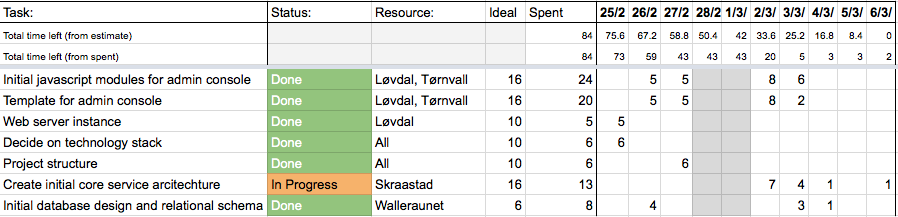
\includegraphics[width=\textwidth]{fig/burndown/sprint1Tasks.png}}
    \caption{Goal achievement for sprint 1}
    \label{fig:sprint 1, goals}
  \end{figure}
\end{center}

\begin{center}
  \begin{figure}[ht!]
    \makebox[\textwidth]{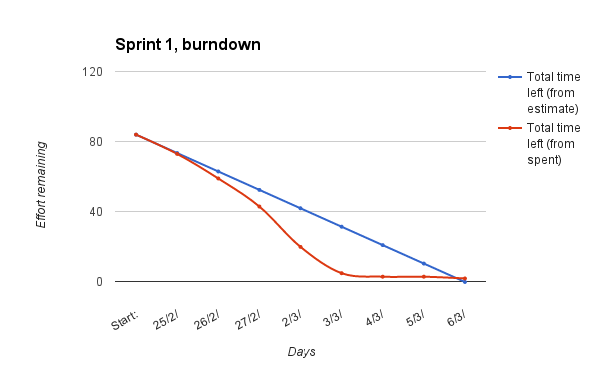
\includegraphics[width=\textwidth]{fig/burndown/sprint1Burndown.png}}
    \caption{Burndown chart for sprint 1}
    \label{fig:sprint 1, burndown}
  \end{figure}
\end{center}

\subsubsection{Discussion}

As expected, the first development sprint was fairly straight forward. The structure of the project was strongly influenced by Apollo. That made the work of defining the structure and base templates simpler, and less time consuming than first expected. Only one of the tasks were still in progress at the end of the sprint. However, given the progress on the task, the group assumed that only a couple of hours remained on it. There were also some minor deviations in the time spent on tasks versus the time that was estimated.

\subsection{Sprint 2}

The major goals of sprint 2 was to get initialize the first draft of the web interface, as well as identify and implement support for processing incoming WSN messages. The midterm report was also due at the end of this sprint.

\subsubsection{Goals}

\begin{center}
  \begin{figure}[ht!]
    \makebox[\textwidth]{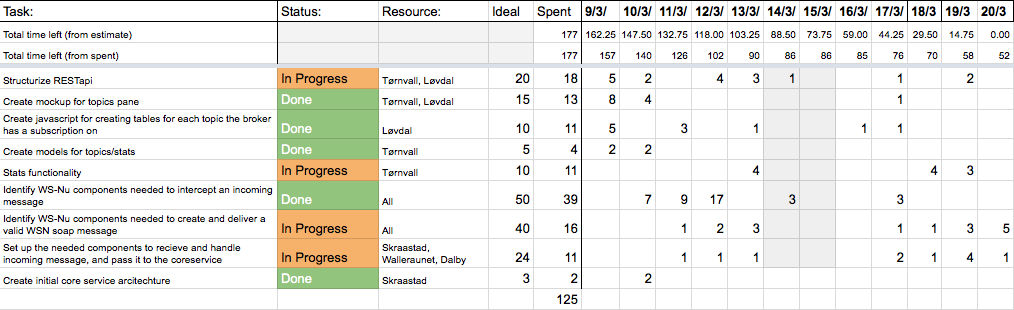
\includegraphics[width=\textwidth]{fig/burndown/sprint2Tasks.png}}
    \caption{Goal achievement for sprint 2}
    \label{fig:sprint 2, goals}
  \end{figure}
\end{center}

\begin{center}
  \begin{figure}[ht!]
    \makebox[\textwidth]{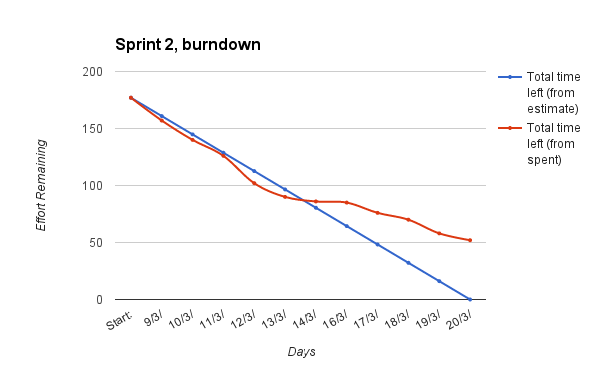
\includegraphics[width=0.9\textwidth]{fig/burndown/sprint2Burndown.png}}
    \caption{Burndown chart for sprint 2}
    \label{fig:sprint 2, burndown}
  \end{figure}
\end{center}

\subsubsection{Discussion}

At the start of this sprint, quite a bit of content lacked on the report in order to deliver a satisfying mid term version. That prompted the group to dedicate a lot of time to the report. Some of the work regarding WSN had to pushed to the next sprint, along with other, less important tasks. Obviously, it would have been preferable to finish the work on time. However, quite a lot of time was left before a functional version of the WSN broker were to be completed. Thus, transferring the packages to the next sprint, seemed okay time-wise. Also, the customer seemed happy with the progress, and was satisfied with the topic handling part of the user interface.

\subsection{Sprint 3}

Only 60 hours were initially scheduled for sprint 3. This was due to Easter, and that three of the group members were on a class trip. The main goals of the sprint were topic and subscription mapping. That included both the logic of it, and passing it to the web interface. The packages from sprint 2 were also included.

\subsubsection{Goals}

\begin{center}
  \begin{figure}[ht!]
    \makebox[\textwidth]{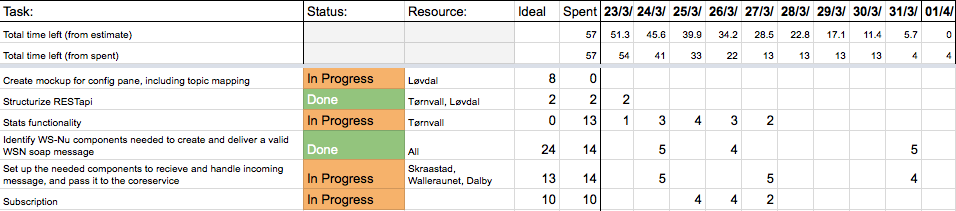
\includegraphics[width=\textwidth]{fig/burndown/sprint3Tasks.png}}
    \caption{Goal achievement for sprint 3}
    \label{fig:sprint 3, goals}
  \end{figure}
\end{center}

\clearpage

\begin{center}
  \begin{figure}[ht!]
    \makebox[\textwidth]{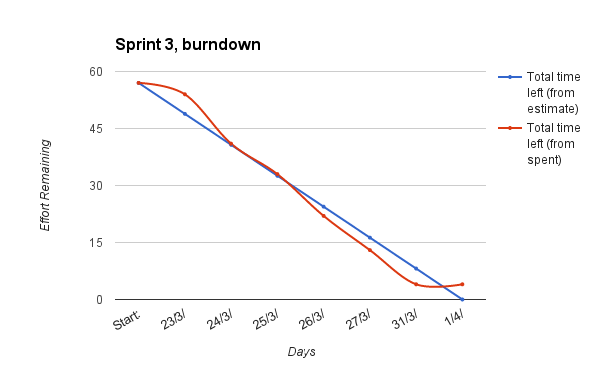
\includegraphics[width=\textwidth]{fig/burndown/sprint3Burndown.png}}
    \caption{Burndown chart for sprint 3}
    \label{fig:sprint 3, burndown}
  \end{figure}
\end{center}

\subsubsection{Discussion}

At this point, the progress and status of the project was not ideal. After the sprint, some of the smaller packages were still unfinished. They were left untouched due to the importance of the other parts of the system. As the system was shaping up as quite complex, more time was used to identify where and how to implement the different parts. This was obviously an issue, as it decreased the amount of code being added. However, the subscription and topic handling were almost completed at the end of the sprint. Thus, no remedial actions were taken at the time, but the issues were kept in mind.


\subsection{Sprint 4}

The focus of this sprint was initially to finalize the implementation of WSN. 87 hours were scheduled due to other courses. Additionally, a lot of work had to be put into the report, the peer evaluation and general research on WSN. The group realized that completing the WSN implementation was not doable at the end of the sprint. The main focus was thus to finalize the subscription and publish parts. Lastly, a major issue with sprint 4 was major deliveries in other courses, that took much more time than anticipated.

\subsubsection{Goals}

\begin{center}
  \begin{figure}[ht!]
    \makebox[\textwidth]{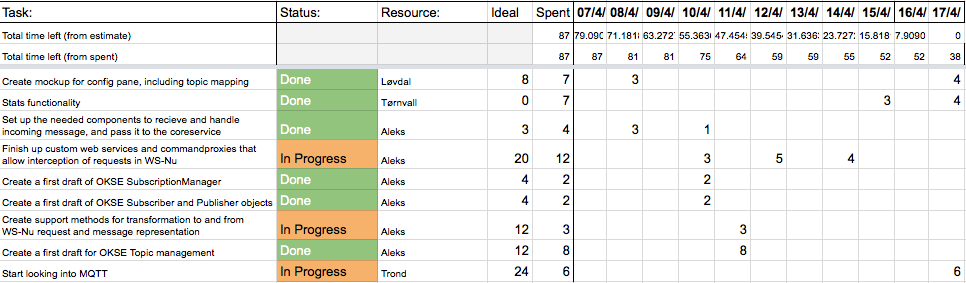
\includegraphics[width=\textwidth]{fig/burndown/sprint4Tasks.png}}
    \caption{Goal achievement for sprint 4}
    \label{fig:sprint 4, goals}
  \end{figure}
\end{center}

\begin{center}
  \begin{figure}[ht!]
    \makebox[\textwidth]{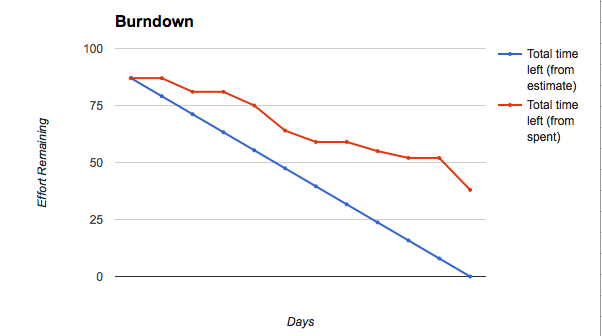
\includegraphics[width=\textwidth]{fig/burndown/sprint4Burndown.png}}
    \caption{Burndown chart for sprint 4}
    \label{fig:sprint 4, burndown}
  \end{figure}
\end{center}

\subsubsection{Discussion}

The two main reasons for this sprint not nearly containing the planned workload were major deliveries in other courses, as well as group members being in Oslo for summer job interviews.
Due to the challenges discussed in the previous sprint, the group had to discuss the priority of requrements with the customer. The solution was to re-prioritize the requirements of MQTT and AMQP support. The result became that AMQP now was the first-in-line protocol to be implemented, bumping MQTT down at a lower priority level. Previously, both AMQP and MQTT had been at the same priority level. That led to a rework of the schedule for the remaining sprints. A lot of time was used for research on the remaining parts of WSN this sprint, along with a lot of report work. WSN proved to be more and more comprehensive and complex, and more code was needed for the implementation than first expected. With this reasoning in mind, the group still somewhat underperformed. Too little time was dedicated to actual development work. Thus, the group realized that a lot more time had to be scheduled for the following sprints. A new work plan was made for the remaining sprints. Deliverables in other courses 

\begin{center}
  \begin{figure}[ht!]
    \makebox[\textwidth]{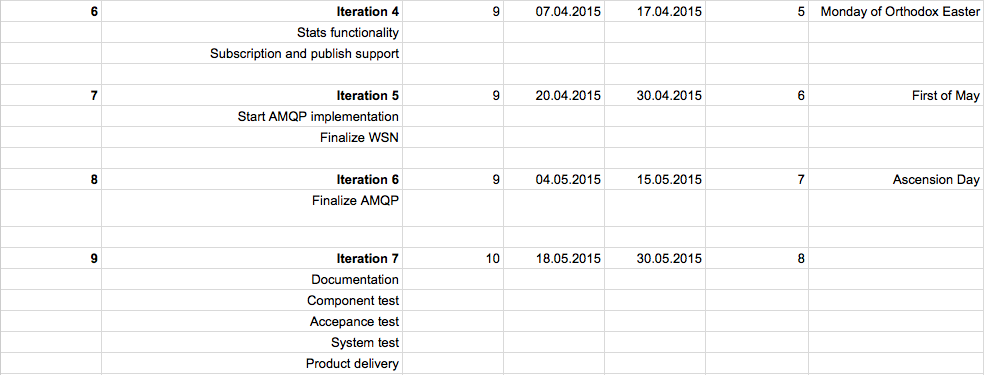
\includegraphics[width=\textwidth]{fig/updatedworkplan.png}}
    \caption{Updated work plan}
    \label{fig:workplan, revised}
  \end{figure}
\end{center}

\subsection{Sprint 5}

\subsubsection{Goals}

\subsubsection{Discussion}

\clearpage